\section*{Contexte et justification du sujet}
Au Burkina Faso, les plantes médicinales occupent une place centrale dans les pratiques de santé. L'Organisation mondiale de la santé rappelle que la médecine traditionnelle demeure, pour une large part des populations des pays en développement, le premier recours de soins \cite{who2013strategy}. Dans le pays, une grande partie de la population, majoritairement rurale, dépend fortement des produits végétaux locaux pour se soigner \cite{zizka_traditional_2015}. Cette importance est reconnue au niveau national, puisque le Ministère de la Santé a engagé un projet d'herbier national dédié aux plantes médicinales, couplé à une chimiothèque de marqueurs chimiques. Ces plantes font par ailleurs l'objet de nombreux travaux scientifiques \cite{ouedraogo_revue_2024}, qui portent sur leurs identifications, leurs usages, leurs propriétés pharmacologiques et leurs toxicités.

Le problème ne vient pas d'un manque de connaissances, mais de leur dispersion. Les informations disponibles sont éparpillées dans la littérature scientifique \cite{zizka_traditional_2015}, notamment dans les articles, les thèses, les mémoires et les rapports de recherche. Or ces documents n'emploient pas les mêmes terminologies. Une même plante y est souvent désignée par plusieurs synonymes ou noms vernaculaires. Il devient alors difficile de comparer les résultats d'une étude à l'autre, de retrouver une information précise sur une plante ou une maladie, et de remonter à la source qui la soutient.

Ce sont des personnes concrètes qui en pâtissent. Le chercheur y perd un temps précieux. L'étudiant ne sait pas toujours à quelle source se fier. Le tradipraticien, qui détient une part de ce savoir, dispose de peu d'outils pour le confronter aux travaux scientifiques. La communauté, qui détient et transmet ces savoirs, n'a pas non plus de moyen simple de les retrouver réunis. Or ces plantes ne sont pas anodines, puisque certaines sont toxiques à forte dose et que la posologie compte. Retrouver, pour chaque information, la source qui la fonde n'est donc pas un luxe de chercheur, mais une condition de confiance.

Les ontologies offrent un moyen de répondre à ce besoin. Elles donnent aux concepts d'un domaine une définition claire et des relations explicites. Les connaissances deviennent alors interopérables et interrogeables \cite{studer1998knowledge}. Dans cette perspective, nous reprendrons un modèle existant consacré aux plantes médicinales, que nous adapterons au contexte burkinabè et enrichirons à partir de la littérature scientifique. Nous utiliserons l'intelligence artificielle pour faciliter l'accès à ces connaissances. Le système interprétera les requêtes en langage naturel, recherchera l'information pertinente dans la base et présentera les résultats de manière accessible. Nous développerons une solution numérique pour servir d'interface entre l'utilisateur et le dispositif. Les réponses seront rattachées aux sources scientifiques correspondantes (figure \ref{fig:rep_connaissances}).

\begin{figure}[H] % H = placement forcé ici (package float)
    \begin{center}
		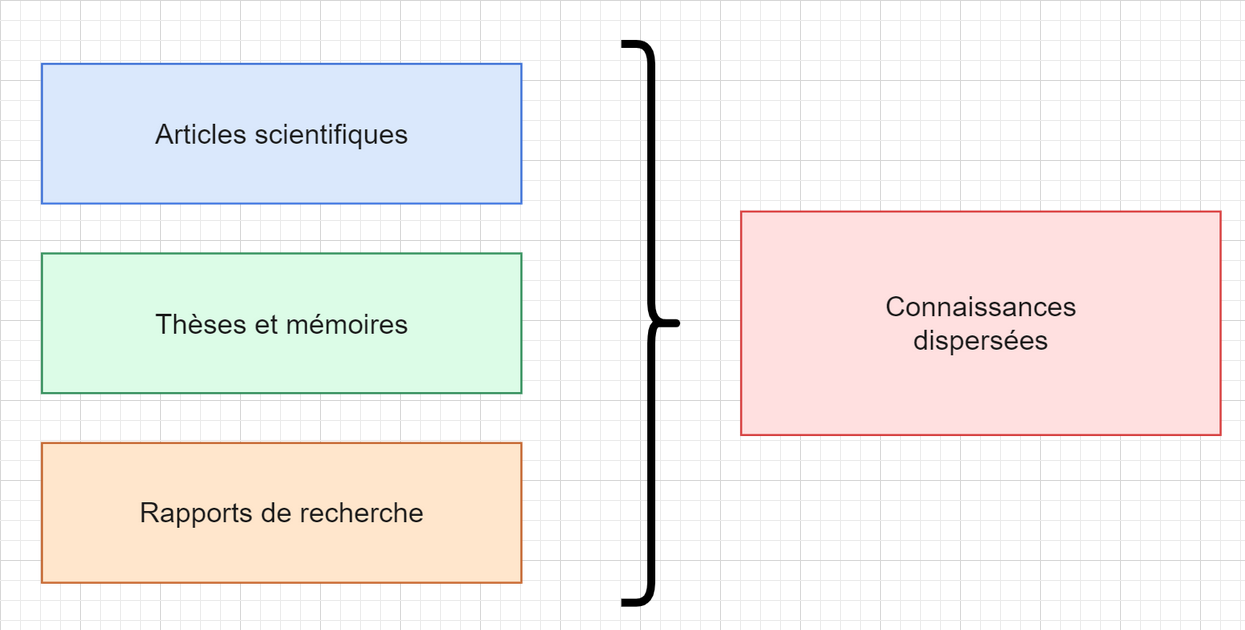
\includegraphics[width=0.8\textwidth]{repartition_connaissances.png}
		\caption{Dispersion des connaissances scientifiques}
		\label{fig:rep_connaissances}
	\end{center}
\end{figure}


\section*{Problématique de la recherche}

Les connaissances scientifiques sur les plantes médicinales du Burkina Faso sont abondantes \cite{ouedraogo_revue_2024} et proviennent de sources variées, comme les articles, les thèses, les mémoires, les rapports de recherche et les bases de données institutionnelles \cite{zizka_traditional_2015}. Leur exploitation pose toutefois problème. Les ontologies peuvent aider à les structurer \cite{shojaee-mend_development_2019}, en représentant les concepts d'un domaine et les relations entre eux, ce qui favorise l'interopérabilité et permet des interrogations plus précises. Comme aucune ontologie ne répond nécessairement aux besoins du contexte burkinabè, nous comparerons les modèles disponibles et retiendrons celui qui conviendra le mieux à l'étude. L'accès constitue une seconde difficulté, car une base structurée peut être riche sans être compréhensible. L'intelligence artificielle pourrait contribuer à réduire cet écart \cite{neha_retrieval-augmented_2025} en interprétant les requêtes en langage naturel, en recherchant les informations pertinentes et en les restituant sous une forme accessible.

Nous étudierons les connaissances issues de la littérature scientifique, leur organisation dans une ontologie adaptée et leur exploitation au moyen de l'intelligence artificielle dans une solution numérique. Notre question principale est la suivante :

\begin{quote}
\textit{Comment réajuster une ontologie existante à partir de la littérature scientifique sur les plantes médicinales du Burkina Faso, puis permettre son interrogation par l'intelligence artificielle afin d'obtenir, en langage naturel, des réponses pertinentes et traçables jusqu'aux sources ?}
\end{quote}

Trois questions spécifiques guideront notre étude :

\begin{itemize}
\item Quelle ontologie existante convient le mieux pour représenter les connaissances sur les plantes médicinales du Burkina Faso, et quels réajustements faut-il lui apporter ?
\item Dans quelle mesure l'intelligence artificielle peut-elle aider à extraire de la littérature scientifique des connaissances fidèles aux documents et rattachées à leurs sources ?
\item Dans quelle mesure une solution numérique interrogeable en langage naturel facilite-t-elle l'accès à ces connaissances pour les chercheurs, les étudiants et les tradipraticiens ?
\end{itemize}

\section*{Objectif général et objectifs spécifiques}

Pour répondre à cette problématique, nous poursuivrons un objectif général, décliné en objectifs spécifiques et en actions évaluables. Ces objectifs guideront notre démarche et nous permettront d'en apprécier les résultats.

\subsection*{Objectif général}

Notre objectif général sera de réajuster une ontologie représentative afin de structurer les connaissances issues de la littérature scientifique sur les plantes médicinales du Burkina Faso, puis d'exploiter ces connaissances au moyen de l'intelligence artificielle et d'une solution numérique pour faciliter leur accès et leur diffusion.

\subsection*{Objectifs spécifiques}

\begin{itemize}
\item Sélectionner, par une étude comparative, l'ontologie la plus adaptée au contexte burkinabè, puis réajuster son modèle conceptuel.
\item Peupler l'ontologie avec des connaissances extraites de la littérature scientifique à l'aide de l'intelligence artificielle, tout en assurant leur traçabilité vers les sources.
\item Développer une solution numérique permettant d'interroger ces connaissances en langage naturel, puis évaluer la qualité de ses réponses.
\end{itemize}

\section*{Hypothèses de recherche}

Pour répondre aux questions posées et atteindre nos objectifs, nous formulerons trois hypothèses. La première portera sur le choix et le réajustement de l'ontologie, la deuxième sur l'extraction des connaissances et la troisième sur l'accès à ces connaissances. Nous les examinerons au cours de la recherche.

\begin{itemize}[label={}, leftmargin=0.5cm]
\item \textbf{Hypothèse 1 :} Une revue méthodique des ontologies existantes permet de sélectionner un modèle qui, après réajustement, représente les connaissances sur les plantes médicinales du Burkina Faso.

\item \textbf{Hypothèse 2 :} L'intelligence artificielle, associée à une vérification manuelle, permet d'extraire de la littérature scientifique des connaissances fidèles aux documents et traçables jusqu'à leurs sources.

\item \textbf{Hypothèse 3 :} Une solution numérique interrogeable en langage naturel devrait faciliter l'accès aux connaissances documentées sur les plantes médicinales du Burkina Faso, avec des réponses pertinentes et sourcées.
\end{itemize}

\section*{Démarche méthodologique adoptée}

Nous suivrons une démarche en six phases, illustrée par la figure \ref{fig:demarche_methodologique}. Après la constitution du corpus, deux volets seront menés en parallèle. Le volet modèle conceptuel sélectionnera puis adaptera l'ontologie ; le volet modèle de données sélectionnera les documents puis en extraira les connaissances. Le modèle adapté fixera le schéma des fiches d'extraction. Les deux volets se rejoindront lors du peuplement de l'ontologie et de la construction de la base de connaissances, sur lesquels reposeront le dispositif numérique puis son évaluation. La démarche articulera la revue de littérature, la comparaison des ontologies, l'ingénierie des connaissances, l'intelligence artificielle et le développement logiciel. Chaque phase donnera lieu à un livrable utile à la suivante. Nous vérifierons les résultats à plusieurs étapes.

\begin{figure}[H]
    \begin{center}
		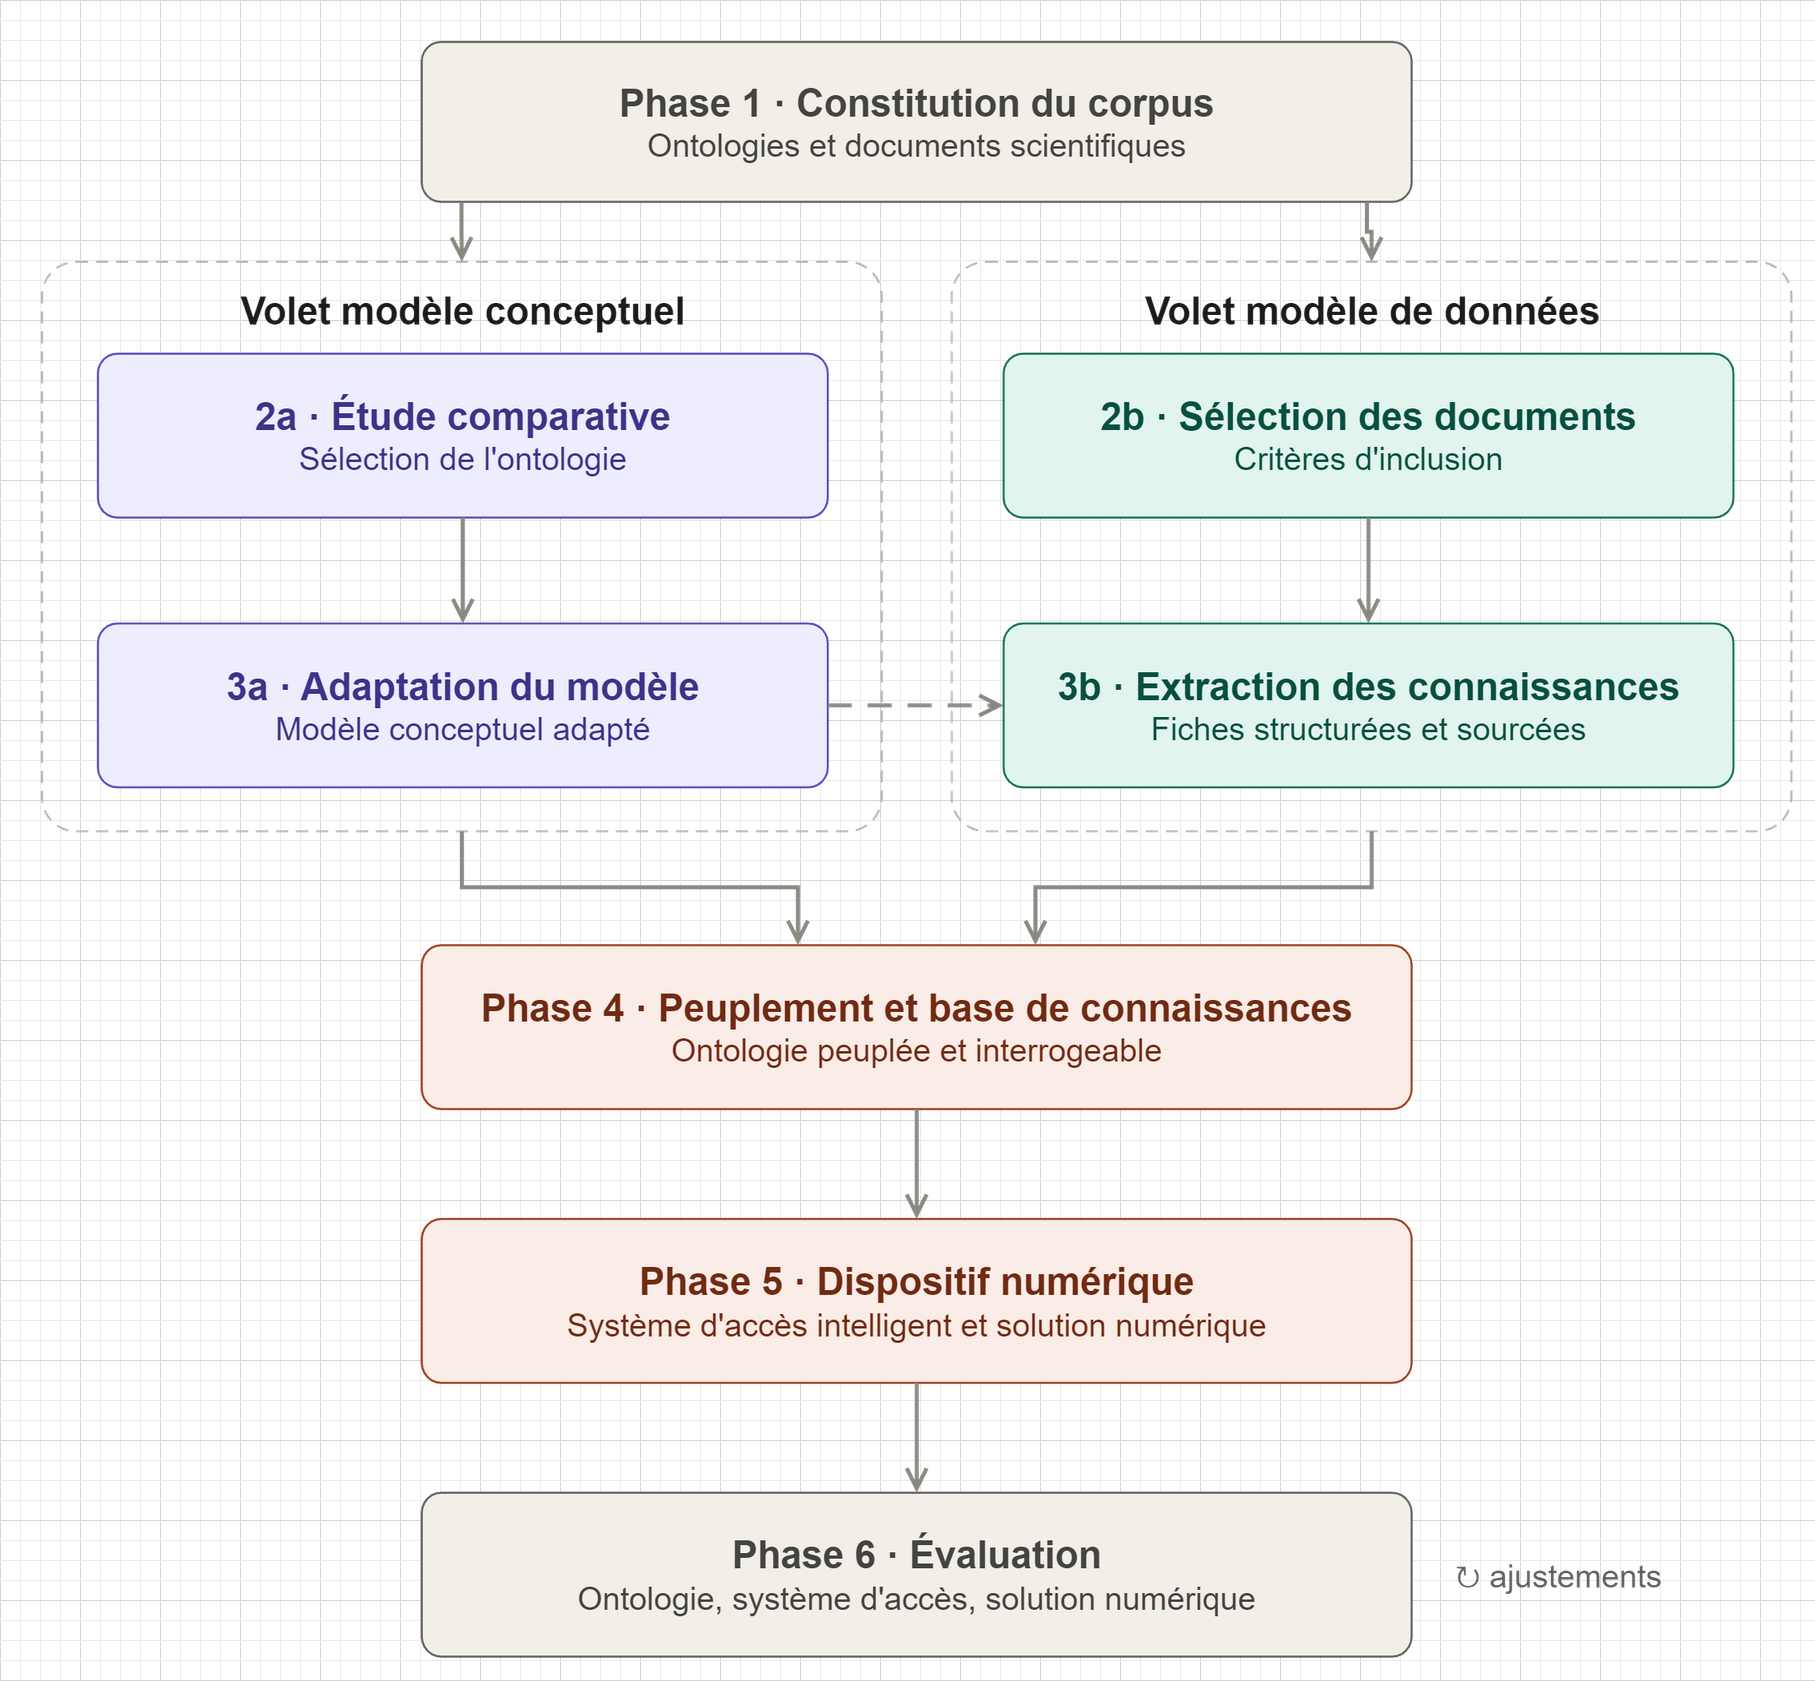
\includegraphics[width=0.8\textwidth]{methodologie_generale.png}
		\caption{Démarche méthodologique adoptée}
		\label{fig:demarche_methodologique}
	\end{center}
\end{figure}

\subsection*{Phase 1 : Constitution du corpus}

Nous rechercherons les ontologies existantes sur les plantes médicinales dans la littérature scientifique et les bases spécialisées. Nous réunirons également les articles, thèses, mémoires et rapports de recherche sur les plantes médicinales du Burkina Faso. La recherche des documents portera sur les plantes, les parties utilisées, les pathologies et usages médicinaux, les modes de préparation, les niveaux de preuve, les propriétés pharmacologiques et la composition chimique. Le livrable sera un corpus réunissant les ontologies candidates et les documents scientifiques collectés.

\subsection*{Volet modèle conceptuel}

\subsubsection*{Phase 2a : Étude comparative des ontologies}

Nous comparerons les ontologies candidates au moyen d'une grille portant sur la couverture du domaine, la richesse sémantique, la disponibilité, la documentation, l'interopérabilité, l'adaptation au contexte burkinabè, la traçabilité et la prise en compte des savoirs locaux. Nous noterons chaque ontologie et retiendrons celle qui obtiendra le meilleur score. Ce choix déterminera le modèle conceptuel des phases suivantes. Le livrable sera l'ontologie sélectionnée.

\subsubsection*{Phase 3a : Adaptation du modèle conceptuel}

Nous adapterons au contexte des plantes médicinales du Burkina Faso le modèle conceptuel de l'ontologie retenue. Nous distinguerons les concepts à conserver, à modifier et à ajouter, notamment pour les maladies, les noms vernaculaires, les régions et les niveaux de preuve, ainsi que les propriétés nécessaires à la localisation et à la traçabilité. Le livrable de cette phase sera le modèle conceptuel adapté, le schéma d'OntoPlantMedBF. Ce schéma fixera aussi les champs des fiches d'extraction de la phase 3b.

\subsection*{Volet modèle de données}

\subsubsection*{Phase 2b : Sélection des documents}

Nous appliquerons aux documents collectés des critères d'inclusion et d'exclusion afin d'en assurer la pertinence, la qualité et la cohérence. Nous examinerons la pertinence du document, l'identification botanique et la disponibilité de références scientifiques vérifiables, puis conserverons la provenance des informations. Nous organiserons et indexerons les documents retenus pour qu'ils servent de base documentaire à notre étude. Le livrable sera le corpus des documents retenus.

\subsubsection*{Phase 3b : Extraction des connaissances}

À partir des documents retenus en phase 2b et selon le schéma défini en phase 3a, nous extrairons les connaissances nécessaires au peuplement de l'ontologie. Nous utiliserons l'intelligence artificielle pour repérer les plantes, leurs usages, les parties utilisées, les préparations et les propriétés pharmacologiques rapportées. Nous structurerons les résultats en fiches et conserverons les références bibliographiques ainsi que, lorsque cela sera possible, les pages ou sections correspondantes. Nous distinguerons les usages rapportés par les enquêtes ethnobotaniques des résultats expérimentaux. Nous reprendrons les niveaux de preuve indiqués par les sources, sans les réévaluer indépendamment. Nous examinerons la qualité des extractions selon le protocole de la phase 6. Le livrable sera un ensemble de fiches structurées et sourcées.

\subsection*{Phase 4 : Peuplement de l'ontologie et construction de la base de connaissances}

Les deux volets se rejoindront dans cette phase. Nous transformerons les fiches en individus du modèle conceptuel adapté, ce qui produira l'ontologie peuplée OntoPlantMedBF. Nous construirons ensuite la base de connaissances en y important cette ontologie, de façon à rendre ses classes, ses propriétés et ses données interrogeables. Le livrable sera l'ontologie peuplée, importée dans une base de connaissances interrogeable.

\subsection*{Phase 5 : Dispositif numérique}

Nous mettrons en place un système d'accès intelligent qui associera la recherche dans la base de connaissances à la génération de réponses par l'intelligence artificielle. Il interprétera les questions en langage naturel, interrogera la base et formulera des réponses accompagnées de leurs sources. Nous développerons une solution numérique proposant une recherche en langage naturel et des fiches sur les plantes, leurs usages, les parties utilisées, les modes de préparation et les références. Le système servira à consulter les connaissances ; il ne posera pas de diagnostic et n'établira pas de prescription. Les livrables seront le système d'accès intelligent et la solution numérique.

\subsection*{Phase 6 : Évaluation}

Nous évaluerons l'approche à trois niveaux. Pour l'ontologie, nous examinerons la couverture, la cohérence, la traçabilité et l'extensibilité. Pour le système d'accès intelligent, nous mesurerons la pertinence, la fidélité, l'exactitude et la traçabilité. Pour la solution numérique, nous mesurerons les performances. Les résultats pourront conduire à des ajustements des phases précédentes, que nous déclarerons avec les mesures qu'ils concernent. Le livrable sera un rapport d'évaluation et de validation.

\section*{Délimitation du champ d'étude}

Notre étude portera sur les plantes médicinales documentées au Burkina Faso et sur les connaissances relatives à leurs usages et à leurs propriétés biologiques rapportés dans les sources scientifiques. Nous nous appuierons sur la littérature accessible et vérifiable, sans mener d'enquête de terrain directe. Nous sélectionnerons une ontologie existante au moyen d'une étude comparative, puis l'adapterons au contexte burkinabè. Sur le plan technique, nous construirons une base de connaissances, mettrons en place un système d'intelligence artificielle pour en faciliter l'accès et développerons une solution numérique. Les consignes données aux outils d'intelligence artificielle faciliteront l'extraction sans constituer des sources scientifiques ; nous nous référerons aux documents eux-mêmes. Le système servira à consulter et à diffuser les connaissances scientifiques. Il ne remplacera pas l'avis d'un professionnel de santé et ne posera pas de diagnostic ni n'établira de prescription.

\section*{Résultats attendus}

Au terme de la recherche, nous prévoyons les résultats suivants :

\begin{itemize}
\item La constitution d'un corpus scientifique organisé sur les plantes médicinales du Burkina Faso, avec les sources et les niveaux de preuve rapportés.
\item La comparaison des ontologies existantes et la sélection de celle qui conviendra à notre étude.
\item L'adaptation de cette ontologie à partir des connaissances issues de la littérature scientifique.
\item La construction d'une base de connaissances et la mise en place d'un système d'accès associant l'intelligence artificielle à la recherche sémantique et à la génération de réponses.
\item Le développement d'une solution numérique qui permettra de rechercher et de consulter les connaissances documentées sur les plantes médicinales du Burkina Faso.
\end{itemize}

\section*{Contribution attendue}

Notre contribution consistera à adapter le modèle conceptuel d'une ontologie sur les plantes médicinales, à enrichir cette ontologie en données issues de la littérature scientifique, puis à importer OntoPlantMedBF dans une base de connaissances. Nous conserverons le lien entre chaque information et sa source. Ce dispositif, complété par un système d'accès intégré à une solution numérique, pourra aider les chercheurs, les étudiants et les autres utilisateurs à consulter les informations documentées, à effectuer des recherches bibliographiques et à explorer les relations entre les plantes et les connaissances scientifiques associées.

\section*{Structuration du mémoire}

Le mémoire est organisé en quatre chapitres numérotés en chiffres romains, précédés de l'introduction générale et suivis de la conclusion générale.

\begin{itemize}
	\item \textbf{Introduction générale (non numérotée).} Le contexte et la justification du sujet y sont exposés, puis la problématique, les questions de recherche, les objectifs et les hypothèses. Y figurent également la démarche méthodologique, la délimitation du champ d'étude et les résultats attendus.

	\item \textbf{Chapitre I :} Cadre théorique et revue de littérature. Les notions liées aux plantes médicinales et aux connaissances scientifiques sur le Burkina Faso y sont présentées, suivies de l'ingénierie des connaissances, des ontologies, des bases de connaissances et de l'intelligence artificielle. Les travaux connexes sont analysés en dernier.

	\item \textbf{Chapitre II :} Matériel et méthodologie. Le corpus scientifique, les critères de sélection et les méthodes d'analyse sont décrits. Les ontologies identifiées, les critères de comparaison, la méthode de sélection et le résultat de la comparaison sont présentés. Les étapes d'adaptation, d'enrichissement et de validation y sont détaillées.

	\item \textbf{Chapitre III :} Conception et développement du système. L'ontologie sélectionnée et les adaptations réalisées y sont présentées, suivies de la base de connaissances, puis de l'intégration de l'intelligence artificielle et du développement de la solution numérique.

\item \textbf{Chapitre IV :} Résultats et discussion. Les résultats de l'évaluation d'OntoPlantMedBF, ontologie adaptée et peuplée, et de la base de connaissances y sont exposés. L'accès intelligent et les fonctionnalités de la solution numérique sont ensuite analysés, et les limites du système discutées.
\end{itemize}

La conclusion générale rappellera les principaux résultats, montrera dans quelle mesure les objectifs et les hypothèses auront été atteints, et présentera les limites du travail ainsi que les perspectives d'amélioration.
